\documentclass{beamer}
\usetheme{Madrid}
\usecolortheme{default}
\usepackage{booktabs} 
\usepackage{multirow} 
\usepackage{tikz} 

\title{Conjugate Gradient in Large-Scale Optimization}
\author{Ronald Nap, Cristian Espinosa}
\date{\today}

\makeatletter
\setbeamertemplate{footline}
{
  \leavevmode
  \hbox{
    \begin{beamercolorbox}[wd=.3\paperwidth,ht=2.5ex,dp=1.125ex,center]{author in head/foot}%
      \usebeamerfont{author in head/foot}Ronald Nap, Cristian Espinosa
    \end{beamercolorbox}
    \begin{beamercolorbox}[wd=.65\paperwidth,ht=2.5ex,dp=1.125ex,right]{title in head/foot}%
      \usebeamerfont{title in head/foot}\inserttitle\hspace*{2em}
    \end{beamercolorbox}
    \begin{beamercolorbox}[wd=0.05\paperwidth,ht=2.5ex,dp=1.125ex,right]{title in head/foot}%
      \usebeamerfont{title in head/foot}\insertframenumber/\inserttotalframenumber\hspace*{2em}
    \end{beamercolorbox}}
  \vskip0pt
}
\makeatother

\begin{document}

\begin{frame}
  \tikz[remember picture,overlay] \node[anchor=north west, inner sep=0pt] at (current page.north west) {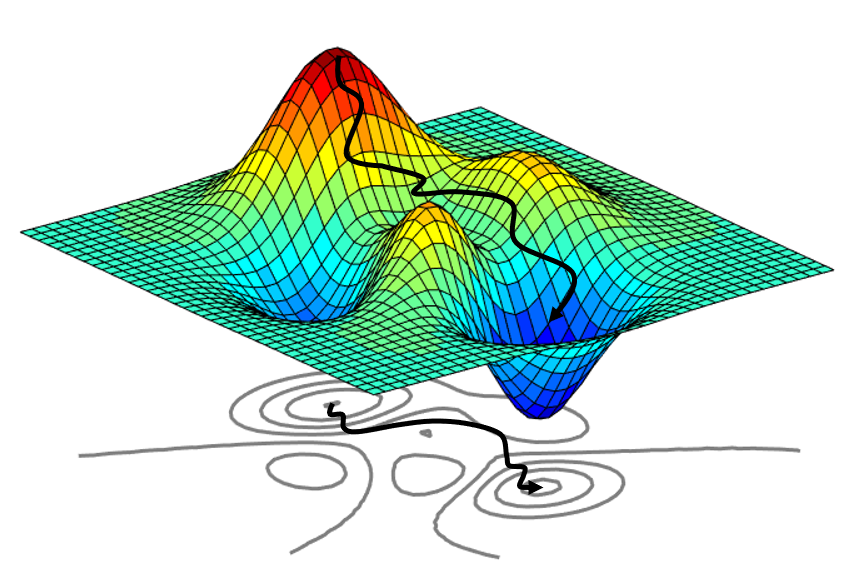
\includegraphics[width=3.5cm]{opt.png}};
  \tikz[remember picture,overlay] \node[anchor=north east, inner sep=0pt] at (current page.north east) {
\includegraphics[width=2.5cm]{ucm.png}};
  \titlepage
\end{frame}


\begin{frame}{Motivation}

      \begin{itemize}
        \item \textbf{Universal Challenge:} Optimization seeks to find the best solution to a problem given some constraints.
        \item \textbf{Broad Applications:} Applications range from machine learning to data mining and image processing.
        \item \textbf{Challenge of Scale:} As datasets grow exponentially, traditional optimization methods struggle to keep up. This drives the need for innovative algorithms that can efficiently handle massive scales of data and high-dimensional spaces without compromising on performance.
      \end{itemize}
    \vspace{-4.5pt}
    \begin{figure}
      \centering
      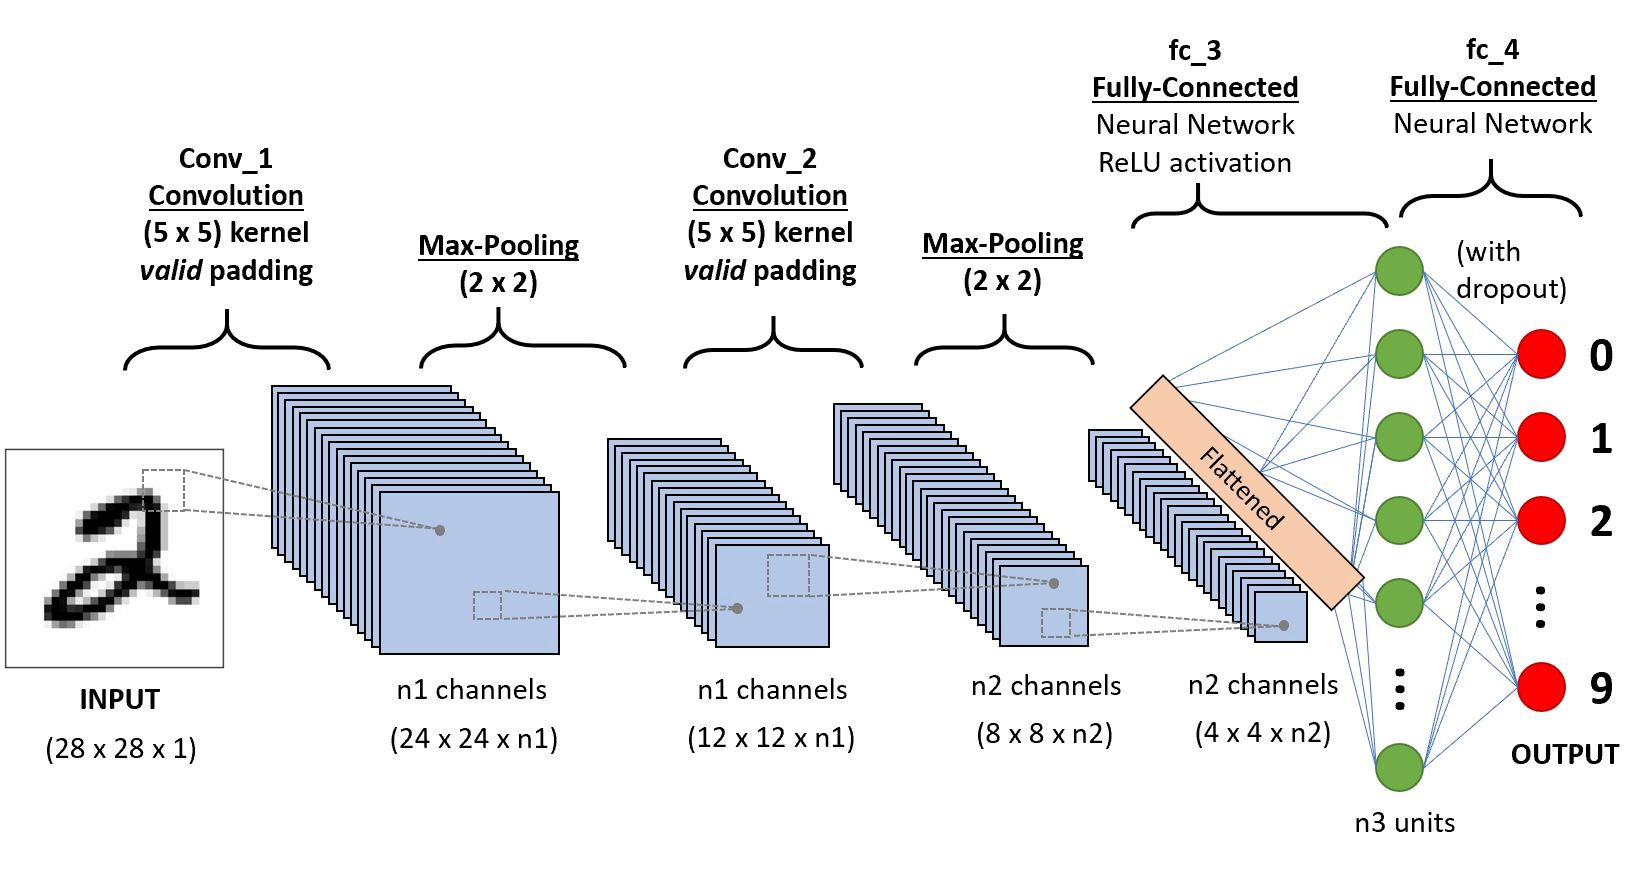
\includegraphics[width=0.8\linewidth, height=0.35\linewidth]{cnn_visual.jpeg}

    \end{figure}
      
\end{frame}



\begin{frame}{Problem Description}
  \footnotesize 

  \begin{block}{Objective}
    The objective is to evaluate the performance of various optimization algorithms taught in class on large-scale problems, comparing their effectiveness to the Conjugate Gradient (CG) method, which is introduced as a suitable algorithm for large-dimensional data.
  \end{block}
  
  \begin{block}{Quadratic Function}
    Defined as \( f(x) = \frac{1}{2} x^T A x - b^T x + c \) where:
    \begin{itemize}
      \item \( A \in \mathbb{R}^{5000 \times 5000} \) is a symmetric positive-definite matrix.
      \item \( b \in \mathbb{R}^{5000} \) is a vector.
      \item \( c \) is a scalar.
    \end{itemize}
  \end{block}
  
  \begin{block}{Rosenbrock Function}
    A non-convex function given by \( g(x) = \sum_{i=1}^{n-1} [100(x_{i+1} - x_i^2)^2 + (1 - x_i)^2] \)
    \begin{itemize}
      \item We test with \( n = 1000 \) to test optimization performance.
    \end{itemize}
  \end{block}
\end{frame}



\begin{frame}{Method}
  \footnotesize 

  \begin{block}{Conjugate Gradient Method}
    \begin{itemize}
      \item Efficiently optimizes quadratic forms, especially when \( A \) is large and sparse.
      \item \textbf{Requirements for Convergence:}
      \begin{itemize}
        \item The matrix \( A \) must be symmetric positive definite.
      \end{itemize}
    \end{itemize}
  \end{block}

  \begin{block}{Pseudocode}
    \begin{enumerate}
      \item Initialize \( x_0 \), compute \( r_0 = b - Ax_0 \), set \( p_0 = r_0 \)
      \item For \( k = 0, 1, 2, \ldots \) until convergence:
      \begin{itemize}
        \item \( \alpha_k = \frac{r_k^T r_k}{p_k^T A p_k} \)
        \item \( x_{k+1} = x_k + \alpha_k p_k \)
        \item \( r_{k+1} = r_k - \alpha_k Ap_k \)
        \item \( p_{k+1} = r_{k+1} + \frac{r_{k+1}^T r_{k+1}}{r_k^T r_k} p_k \)
      \end{itemize}
    \end{enumerate}
  \end{block}
\end{frame}



\begin{frame}{Conjugate Gradient Method: Pros and Cons}
  \begin{columns}[T] 
    \begin{column}{0.5\textwidth}
      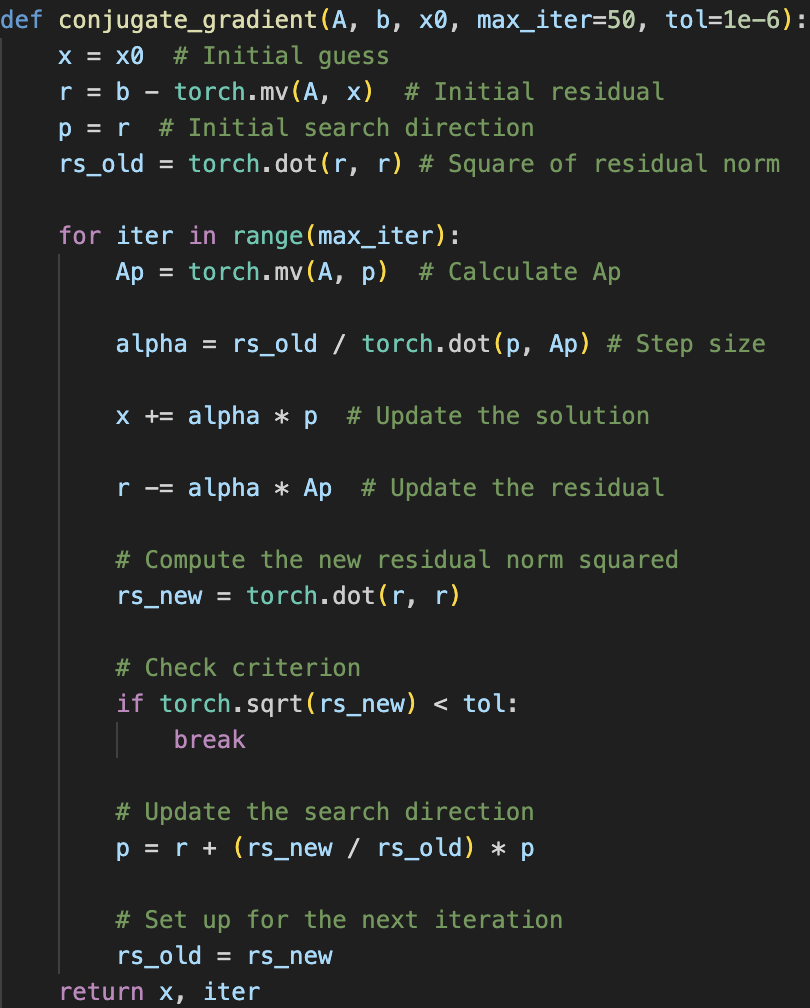
\includegraphics[width=\linewidth]{cg.png}
    \end{column}

    \begin{column}{0.5\textwidth}
      \footnotesize 
      \begin{block}{Pros}
        \begin{itemize}
          \item Efficiently handles large, sparse matrices
          \item Only requires matrix-vector products
          \item No need for matrix storage
          \item Potentially faster than other methods for certain problems
        \end{itemize}
      \end{block}

      \begin{block}{Cons}
        \begin{itemize}
          \item Convergence can be slow for ill-conditioned systems
          \item Performance is heavily dependent on preconditioning
          \item Not as robust as more modern algorithms in certain contexts
        \end{itemize}
      \end{block}
      \normalsize
    \end{column}
  \end{columns}
\end{frame}

\begin{frame}{Preconditioning}
  \footnotesize 
    \begin{block}{Preconditioning and Condition Number}
        Preconditioning (1) is a technique used to transform a given problem into a form that is more amenable to numerical methods. It involves modifying the system of equations:
    \begin{align*}
        Ax &= b \quad \text{to} \quad M^{-1}Ax = M^{-1}b \qquad \text{(1)} & \quad \kappa(A) = \frac{\lambda_{\max}}{\lambda_{\min}} \qquad \text{(2)}
    \end{align*}
        
        where \( M \) is the preconditioner. The objective is to select a preconditioner \( M \) so that \( M^{-1}A \) possesses a lower condition number compared to \( A \). The condition number given by (2) quantifies the numerical instability when solving \( Ax = b \).        

  \begin{itemize}
    \item \textbf{Solving \(Ax = b\):} The CG method efficiently solves the equation \(Ax = b\), where \(A\) is a symmetric positive definite. This method iteratively approaches the solution by minimizing the residual, which depends crucially on the characteristics of \(A\).

    \item \textbf{Digits of Accuracy:} The number of digits of accuracy achievable is given by:
      \[
      \text{Digits of Accuracy} \approx -\log_{10}(\kappa(A))  \qquad \text{(3)}
      \] 
      This formula implies that a higher condition number results in fewer digits of accuracy in the solution, underscoring the need for a low condition number.
  \end{itemize}

\end{block}

  \normalsize 
\end{frame}


\begin{frame}{Review of Optimization Methods}
  \footnotesize 
  \begin{table}
  \centering
  \begin{tabular}{|p{0.09\textwidth}|p{0.35\textwidth}|p{0.25\textwidth}|p{0.14\textwidth}|}
    \hline
    \textbf{Method} & \textbf{Pros} & \textbf{Cons} & \textbf{Convergence} \\
    \hline
    Steepest\newline Descent & -Requires only function and gradient evaluations & Slow convergence & Linear \\
    \hline
    Newton's\newline Method & -Quadratic convergence \newline -Handles non-linear problems & Requires second-order derivatives; computation heavy for large systems & Quadratic  \\
    \hline
    Trust\newline Region & -Robust;  \newline -Handles non-linear problems; \newline -Does not rely on line search & -More parameters to tune; \newline -Requires Hessian or its approximation & Superlinear \\
    \hline
    BFGS & -Avoids Hessian computation using secant updates; -Good practical performance & -High memory needed; -Convergence not guaranteed for non-convex functions & Superlinear \\
    \hline
  \end{tabular}
  \end{table}
\end{frame}


\begin{frame}{Numerical Results}
  \footnotesize 
  \begin{table}
    \centering
    \begin{tabular}{@{}lcccc@{}}
      \toprule
      \textbf{Function} & \textbf{Method} & \textbf{Iterations} & \textbf{Time (s)} & \textbf{Rel. Error} \\
      \midrule
      \multirow{8}{*}{Quadratic} & Conjugate Gradient & 3 & \textbf{0.0088} & $5.81 \times 10^{-7}$ \\
                                 & Preconditioned CG & 2 & 1.4007 & $3.12 \times 10^{-9}$ \\
                                 & Steepest Descent & 50 & 7.9327 & $6.71 \times 10^{-7}$ \\
                                 & Newton's Method & 2 & 1.1769 & \boldmath{$3.59 \times 10^{-15}$} \\
                                 & BFGS & 5 & 87.0257 & $1.71 \times 10^{-7}$ \\
                                 & Trust Region & 50 & 139.0355 & $7.32 \times 10^{-7}$ \\
                                 & Trust Region + CG & 50 & 0.7868 & $1.44 \times 10^{-7}$ \\
      \midrule
      \multirow{8}{*}{Rosenbrock} & Conjugate Gradient & 2 & \textbf{0.0046} & $0.999$ \\
                                  & Preconditioned CG & 2 & 0.2504 & $0.999$ \\
                                  & Steepest Descent & 50 & 19.0641 & $0.916$ \\
                                  & Newton's Method & 50 & 44.8113 & $0.657$ \\
                                  & BFGS & 50 & 29.2694 & $0.979$ \\
                                  & Trust Region & 50 & 11.8806 & \textbf{0.575} \\
                                  & Trust Region + CG & 50 & 4.4343 & \textbf{$0.726$} \\
      \bottomrule
    \end{tabular}
  \end{table}
  \normalsize 
\end{frame}


\begin{frame}{Discussion of Numerical Results}
  \footnotesize

  \begin{block}{Key Findings}
    \begin{itemize}
      \item \textbf{Efficiency:} Conjugate Gradient stands out in both functions for significantly reducing the number of iterations and computational time.
      \item \textbf{Accuracy:} Newton's Method achieves the lowest relative error for the quadratic function and obtained the secondest lowest relative error on the rosenbrock function demonstrating high accuracy despite higher computational time.
      \item \textbf{Trade-offs:} BFGS and Steepest Descent show mixed results, Trust Region demonstrates efficiency and relatively low error, suggesting a balanced approach.

    \end{itemize}
  \end{block}

  \begin{block}{Implications}
    \begin{itemize}
      \item The choice of optimization method should consider the specific demands of the problem, weighing the need for speed against accuracy.
      \item For rapid convergence in less complex or well-conditioned problems, Conjugate Gradient might be preferable, while Newton's Method is recommended for situations where high accuracy is critical.
      \item Trust Region + CG could be a versatile choice, offering a good compromise between convergence speed and accuracy.
    \end{itemize}
  \end{block}

  \normalsize
\end{frame}
\end{document}